\begin{frame}
\frametitle{Многоуровневая организация памяти}
\begin{center}
  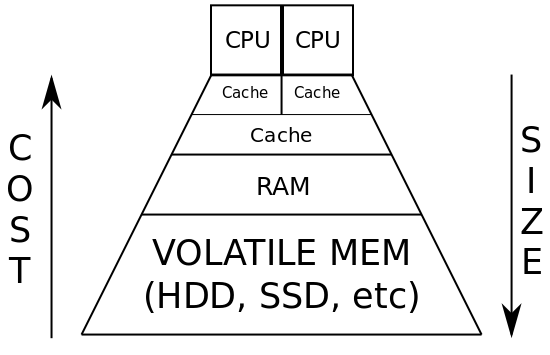
\includegraphics[width=0.6\linewidth]{hierarchy.png}
\end{center}
\begin{itemize}
  \item CPU очень быстрый, а память либо медленная либо дорогая
  \begin{itemize}
    \item поэтому приходится использовать несколько уровней памяти;
    \item чем ближе память к процессору, тем она быстрее и тем ее меньше;
  \end{itemize}
\end{itemize}
\end{frame}

\begin{frame}
\frametitle{Принцип локальности}
\begin{itemize}
  \item Временная локальность:
  \begin{itemize}
    \item когда программа обращается к одним и тем же данным в течение короткого
    интервала времени;
    \item пример: цикл считающий сумму элементов массива - переменная с
    результатом обновляется на каждый элемент массива.
  \end{itemize}
  \item Пространственная локальность:
  \begin{itemize}
    \item когда программа обращается к близким ячейкам памяти в течение
    короткого интервала времени;
    \item пример: цикл считающий сумму элементов массива - мы читаем элементы
    массива последовательно.
  \end{itemize}
  \item Зачастую, ваша программа не работает сразу со всеми петабайтами данных
  одновременно.
\end{itemize}
\end{frame}

\begin{frame}
\frametitle{Когерентность кешей}
\begin{itemize}
  \item CPU, зачастую, имеет свой собственный кеш:
  \begin{itemize}
    \item что если два CPU в своих кешах закеширвоали одну и ту же переменную?
    \item ничего плохого, пока копии идентичны;
    \item что если один из CPU решил обновить значение у себя в кеше?
    \item одна и та же переменная будет иметь разные значения для разных CPU.
  \end{itemize}
  \item Архитектуры, которые разрешают кешам "расходиться" называются
  некогерентными
  \begin{itemize}
    \item не менстрим.
  \end{itemize}
\end{itemize}
\end{frame}

\begin{frame}
\frametitle{Протоколы когерентности кешей}
\begin{itemize}
  \item Для обеспечения когерентности кеши могут обмениваться сообщениями
  \begin{itemize}
    \item CPU соединены между собой полноценной сетью;
    \item не такой как TCP/IP/Ethernet, но все еще полноценной.
  \end{itemize}
  \item Классы сообщений и как нужно на них реагировать - протокол когерентности
  кешей
  \begin{itemize}
    \item классический \emph{учебный} пример - протокол MESI.
  \end{itemize}
\end{itemize}
\end{frame}

\begin{frame}
\frametitle{Протокол MESI 1/3}
\begin{itemize}
  \item Каждая кеш-линия имеет одно из следующих состояний:
  \begin{itemize}
    \item M (Modified) - версия данных в кеш линии отличается от того, что
    хранится в памяти, а кроме того данный кеш является \emph{единственным}
    владельцем данных;
    \item E (Exclusive) - версия данных в кеш линии совпадает с тем, что
    хранится в памяти, и данный кеш \emph{единственный} владелец данных;
    \item S (Shared) - версия данных может находится в других кешах, и совпадает
    с тем, что хранится в памяти;
    \item I (Invalid) - кеш линия не хранит данных.
  \end{itemize}
\end{itemize}
\end{frame}

\begin{frame}
\frametitle{Протокол MESI 2/3}
\begin{itemize}
  \item Кеши и память обмениваются друг с другом сообщениями:
  \begin{itemize}
    \item мы считаем все сообщения широковещательными, т. е. каждый видит все
    сообщения.
  \end{itemize}
  \item Состояние кеш линии, обычно, меняется в ответ на получение сообщения.
  \item Modified может измениться в Exclusive, если процессор решил обновить
  версию в памяти
  \begin{itemize}
    \item кеш имеет ограниченный размер и когда-то мы должны из него что-то
    выбросить;
    \item если кеш хранит более новую версию чем память, то перед тем как
    выбрасить ее из кеша нужно обновить память;
    \item любую кеш линии в состоянии S или E можно спокойно выбрасывать из
    кеша.
  \end{itemize}
\end{itemize}
\end{frame}

\begin{frame}
\frametitle{Протокол MESI 3/3}
\begin{itemize}
  \item Типы сообщений:
  \begin{itemize}
    \item Read - у нас в кеше нет данных, мы хотим прочитать их из памяти или
    другого кеша;
    \item Read Response - ответ на запрос Read, вообще говоря, ответить может
    кто угодно, но мы будем считать, что отвечает всегда кеш, в котором есть
    данные или память, если кеша с новой версией данных не нашлось;
    \item Invalidate - заставить все кеши сбросить свою версию определенных
    данных;
    \item Invalidate Ack - подтверждение, что другие кеши сбросили свою версию
    данных, только получив подтверждение мы можем двигаться дальше;
    \item Read Invalidate - Read и Invalidate вместе, т. е. не только дайте мне
    данные, но еще и удалите их у себя.
  \end{itemize}
\end{itemize}
\end{frame}

\begin{frame}
\frametitle{Финальные замечания про когерентность кешей}
\begin{itemize}
  \item Фактически, чтобы обновить разделяемые данные необходимо быть их
  единственным владельцем:
  \begin{itemize}
    \item перед тем, как мы сможем обновить данные в кеше, кеш линия должна быть
    в состоянии E или M;
    \item запись в общие данные приводит к обмену сообщениями, ожиданию ответов
    и поэтому стоит дорого;
    \item нужно избегать записи в одну и ту же переменную с разных CPU, или
    ограничивать количество CPU пишущих в одну переменную;
    \item другими словами нужно избегать активной конкуренции (contention).
  \end{itemize}
\end{itemize}
\end{frame}
